\documentclass[12pt,a4paper]{amsart}
\usepackage[UTF8]{ctex}
\usepackage{preamble}
\usepackage{booktabs} % 添加 booktabs 宏包

\title{实验报告:阻尼振动和受迫振动}

\begin{document}

\maketitle

\section{实验小结}

\subsection{数据记录}

\subsubsection{定性观察弦的振动,研究 f 和 N 关系}

\begin{table}[H]
    \centering
    \caption{定性观察弦的振动,研究 f 和 N 关系}
    \begin{tabular}{cc} % 修改此处的列格式
        \toprule
        N & f \\            
        \midrule
        1 & 33.34 Hz \\
        2 & 66.76 Hz \\
        3 & 100.08 Hz \\
        4 & 133.42 Hz \\
        \bottomrule
    \end{tabular}
    \label{chart}
\end{table}

\subsubsection{定性观察弦的振动,研究 f 和 L 关系}

\begin{table}[H]
    \centering
    \caption{定性观察弦的振动,研究 f 和 L 关系}
    \begin{tabular}{cc} % 修改此处的列格式
        \toprule
        L & f \\            
        \midrule
        30cm & 112.27 Hz \\
        35cm & 98.34 Hz \\
        40cm & 86.40 Hz \\
        45cm & 78.56 Hz \\
        50cm & 69.87 Hz \\
        55cm & 64.01 Hz \\
        \bottomrule
    \end{tabular}
    \label{chart}
\end{table}

\subsubsection{测量 f 和 T 关系}

\begin{table}[H]
    \centering
    \caption{测量 f 和 T 关系}
    \begin{tabular}{cc}
        \toprule
        T & f \\
        \midrule
        1.96 N & 44.72 Hz \\
        3.92 N & 63.30 Hz \\
        5.88 N & 77.60 Hz \\
        7.84 N & 89.36 Hz \\
        9.80 N & 100.01 Hz \\
        11.76 N & 109.92 Hz \\
        \bottomrule
    \end{tabular}
    \label{chart}
\end{table}

\subsubsection{测量 f 和 $\rho$ 关系}

\begin{table}[H]
    \centering
    \caption{测量 f 和 $\rho$ 关系}
    \begin{tabular}{cc}
        \toprule
        $\rho$ & f \\
        \midrule
        $\rho_1$ & 133.60 Hz \\
        $\rho_2$ & 100.01 Hz \\
        $\rho_3$ & 71.78 Hz \\
        $\rho_4$ & 53.12 Hz \\
        $\rho_5$ & 41.20 Hz \\
        $\rho_6$ & 32.67 Hz \\
        \bottomrule
    \end{tabular}
    \label{chart}
\end{table}

\subsubsection{研究弦线的线密度、弦长、张力、基频与波速的关系}

\begin{table}[H]
    \centering
    \caption{研究弦线的线密度、弦长、张力、基频与波速的关系}
    \begin{tabular}{ccc}
        \toprule
        N & 理论 & 实际 \\
        \midrule
        1 & 133.48 Hz & 133.60 Hz \\
        2 & 100.00 Hz & 100.01 Hz \\
        3 & 71.63 Hz & 71.78 Hz \\
        4 & 52.92 Hz & 53.12 Hz \\
        5 & 41.18 Hz & 41.20 Hz \\
        6 & 32.35 Hz & 32.67 Hz \\
        \bottomrule
    \end{tabular}
    \label{chart}
\end{table}

\subsection{实验结论}

通过实验,我们验证了以下弦振动公式

\begin{equation}
    f = \frac{1}{2L} \sqrt{\frac{T}{\rho}}
\end{equation}

\section{原始数据}

\begin{figure}[h]
	\centering
	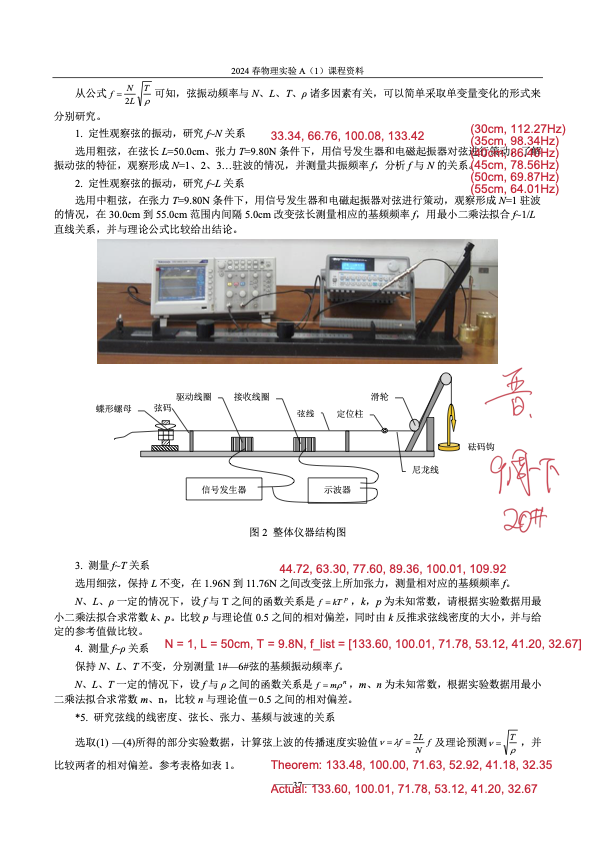
\includegraphics[width=1.0\textwidth]{img/original_data.png}
	\caption{原始数据记录页}
	\label{fig:original_data_page_1}
\end{figure}

\end{document}
